\begin{sidewaysfigure}
  \centering
  \begin{minipage}{.8\textwidth} % adjust the width as needed

    \begin{minipage}{\textwidth}
      \centering
      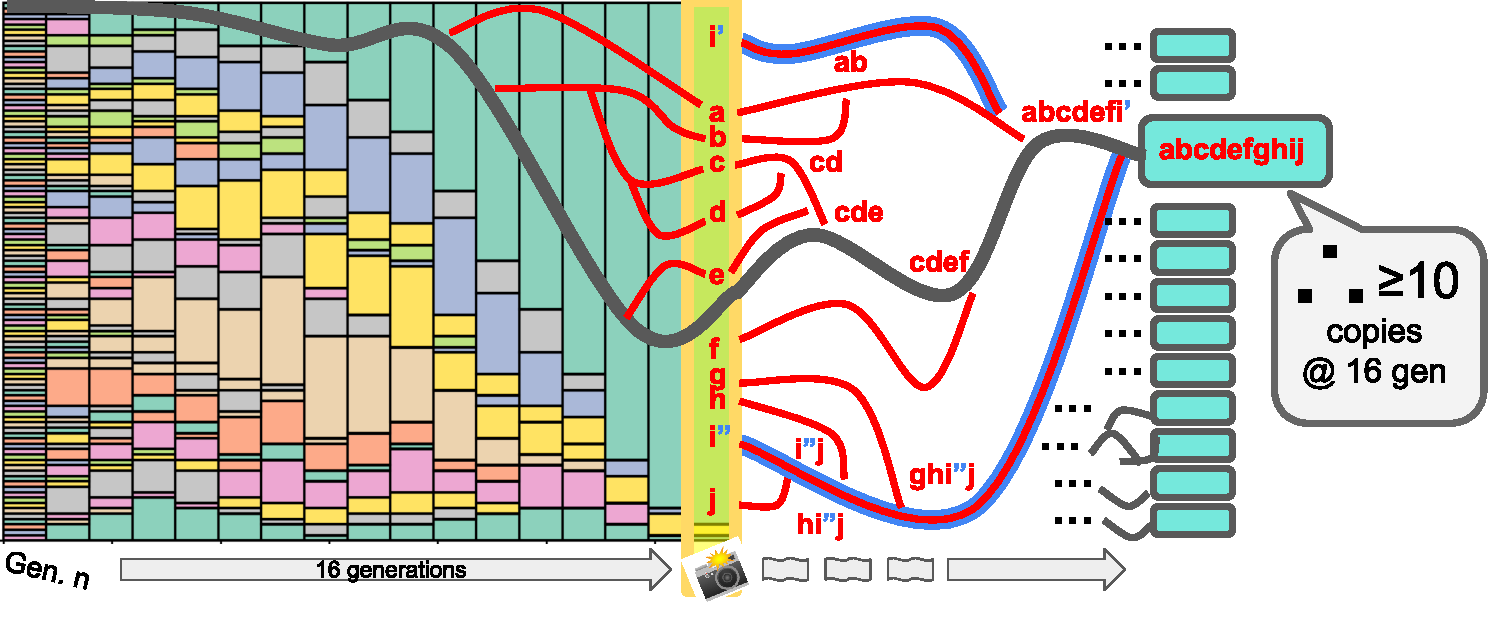
\includegraphics[height=0.4\textheight]{img/copy-count-snapshot}
      \subcaption{TODO}
      \label{fig:ne-example-replicates:bottleneck}
    \end{minipage}%

    \vspace{1cm}

    \begin{minipage}{0.5\textwidth}
      \centering
      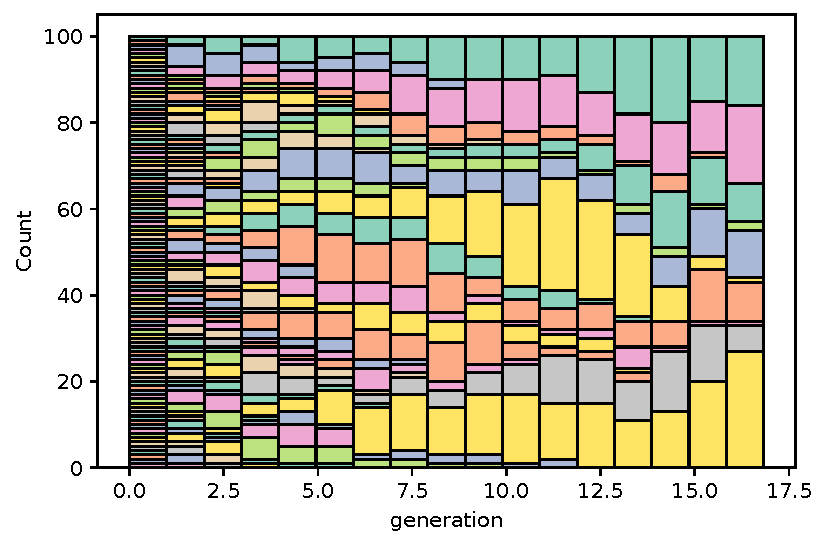
\includegraphics[height=0.25\textheight]{notebooks/notebooks/teeplots/fit=0.0+hue=clade+multiple=stack+ngen=16+npop=100+palette=set2+viz=histplot+x=generation+ext=}
      \subcaption{Selection pressure treatment}
      \label{fig:ne-example-replicates:selection_pressure}
    \end{minipage}%
    \begin{minipage}{0.5\textwidth}
      \centering
      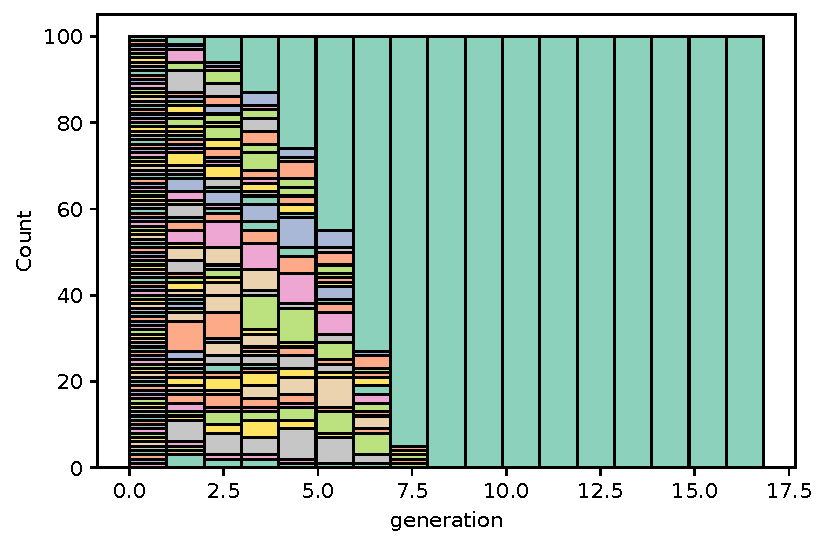
\includegraphics[height=0.25\textheight]{notebooks/notebooks/teeplots/fit=1.0+hue=clade+multiple=stack+ngen=16+npop=100+palette=set2+viz=histplot+x=generation+ext=}
      \subcaption{TODO}
      \label{fig:ne-example-replicates:control}
    \end{minipage}

  \end{minipage}
  \hfill % Creates horizontal space. Can also use \hspace{<len>}
  \begin{minipage}{.15\textwidth} % adjust the width as needed
    \caption{TODO
    }
    \label{fig:ne-example-replicates}
  \end{minipage}

\end{sidewaysfigure}


% notebooks/notebooks/teeplots/notebook=ne-inference+replicate=0+treatment=bottleneck+viz=plot-running-estimation+x=rank+y=population-size+ext=.pdf
%
% notebooks/notebooks/teeplots/notebook=ne-inference+replicate=0+treatment=control+viz=plot-running-estimation+x=rank+y=population-size+ext=.pdf
%
% notebooks/notebooks/teeplots/notebook=ne-inference+replicate=0+treatment=range-expansion+viz=plot-running-estimation+x=rank+y=population-size+ext=.pdf
%
% notebooks/notebooks/teeplots/notebook=ne-inference+replicate=0+treatment=selection-pressure+viz=plot-running-estimation+x=rank+y=population-size+ext=.pdf
